% Appendix: the trained controller (docs/TRAINED_BASELINE.md: plan, code and reading rules written 9 Nov 2026 02:27
% UTC and sent for a timestamp before training started; deviations 1-3 logged there). Code: policies/trained_residual.py,
% sb/train_rl.py, sb/rl_core.py; test: sb/run_trained.py (results/rl_test, summary.json); figure: sb/fig_trained.py.
% The budget numbers come from results/rl/main/train.csv via summary.json; fill them when training has ended.
\section{A trained controller}\label{app:trained}
The starter kit ships no trained policy, so we trained one to compare with. It is a residual on pid\_water: it adds
corrections to the baseline's commands and, with zero weights, reproduces pid\_water action for action (checked over
360 steps), so training starts from the strongest official baseline. One network (27 inputs, two hidden layers of 64
tanh units) is shared by all zones and corrects each zone's damper and reheat commands; a second one of the same shape
is shared by all air handlers and corrects supply-air temperature, fan pressure and recirculation. Shared weights let
the policy run in any building, of any size. It decides every 15 minutes; the on/off commands and the hot-water loop
stay with pid\_water. A zone's inputs are its temperature relative to the comfort band and to the band in force, its
last two changes, the clock and comfort flags, the hours to the comfort period, the outside temperature and its
24-hour mean, the building's occupancy, the last commands, the box size, the air handler's state and the baseline's
own command. Nothing from v16 goes in: no zone model and no delay handling.

We trained it with PPO, in our own numpy code (every gradient checked against finite differences), on the 25 scenarios
of five training buildings. Each zone has its own reward, its comfort term plus its share of the energy and carbon
cost, scaled so that the mean over zones is the building's reward; each air handler takes the mean over its zones. The
sixth training building (building\_train\_4, five scenarios) only chose the checkpoint, by the mean loss over 2880 steps
without exploration noise. Training ran on our copy of the simulator with both proposed energy fixes (Appendix~\ref{app:tank}),
so the policy cannot learn the hot-water accounting issue; the test ran on the shipped simulator, as every other result
in this paper. The budget was 3.3 million simulator steps in 38 hours on three CPU processes: one
architecture, one budget, one seed. Three changes during training are logged with the plan. All came before any test
run and were decided on training and validation data only. First, smaller minibatches after 3.9 hours. Second,
validation every 100 instead of 150 iterations. Third, after the validation loss rose from iteration 450 on, a restart
from that checkpoint with shorter episodes, a lower learning rate and averaged weights (Figure~\ref{fig:trained}). The
chosen checkpoint, iteration 1200, has a validation loss of 0.02339 against pid\_water's 0.03293.

\begin{figure}[!htb]\centering
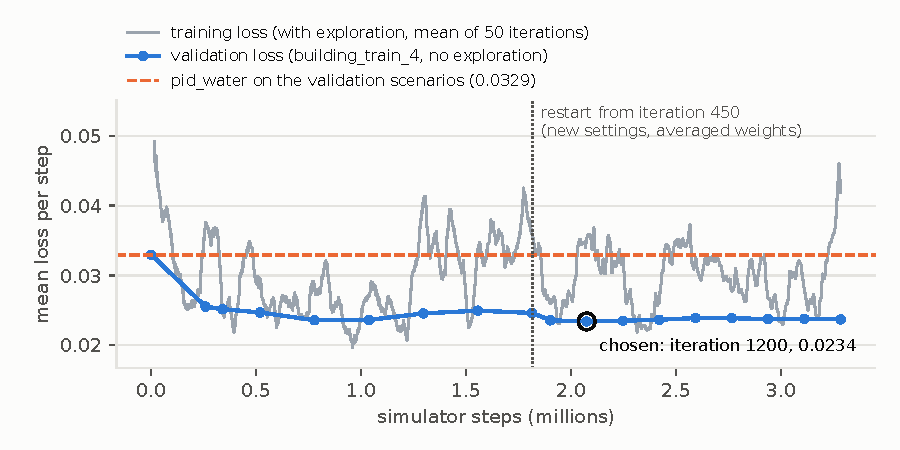
\includegraphics[width=0.86\linewidth]{../docs/fig/fig_trained.pdf}
\caption{Training of the residual controller: loss on the validation building (five scenarios, 2880 steps, no
exploration noise; corrected simulator) and the training loss (with exploration noise, mean of 50 iterations), against
simulator steps. Dashed: pid\_water on the validation scenarios.}
\label{fig:trained}
\end{figure}

\begin{table}[!htb]\centering
\caption{The trained controller on the twelve full-size buildings of rounds 6 and 7 (first 2880 steps each, shipped
simulator; the buildings of Table~\ref{tab:what}), tested once after training. Loss: mean loss per step; Comfort: mean
comfort term per step; ratio of mean losses with a 95\,\% bootstrap interval over scenarios.}\label{tab:trained}
\small
% Written by sb/run_trained.py --read from results/rl_test (do not edit by hand).
\begin{tabular}{llcccc}\toprule
Policy & Training & Loss & Comfort & Loss / pid\_water & Below pid\_water\\\midrule
pid\_water & none (official baseline) & 0.07982 & 0.06341 & 1 & --\\
trained residual & 38\,h, 3.3\,M steps & 0.07141 & 0.06016 & 0.89 (0.83--0.95) & 11 of 12\\
v16 & none (learns online) & 0.01427 & 0.00048 & 0.18 (0.13--0.24) & 12 of 12\\\bottomrule
\end{tabular}

\end{table}

% Reading rules of docs/TRAINED_BASELINE.md, fixed before training.
The rules fixed before training define a real improvement on pid\_water: at most 0.95 times its loss, and a lower
loss in at least 9 of 12 scenarios. The trained policy reached 0.89 times (95\,\% interval 0.83--0.95) and was lower in
11 of 12, so it is one. v16 beats it with this budget: v16 is lower in 12 of 12, and the trained policy's loss is 5.0
times v16's (interval 3.5--7.3). The trained policy's gain over pid\_water is energy. The energy and carbon part of its
loss is 0.69 times pid\_water's (0.82 times v16's), but its comfort term stays at 0.95 times pid\_water's, while v16's
is under 1\,\% of it (Table~\ref{tab:trained}). On the validation building, of the shipped size, it had reached 0.71 times
pid\_water's loss. Before the test we expected 0.6--1.0 times pid\_water's loss and a factor of 3--5 to v16 (our
opinion, written in the plan). Both drew on the same six shipped buildings: v16's design during development, the
trained policy for training and validation. One architecture, one budget and one seed say little about what trained
control can reach.

% Kaggle public leaderboard, one submission of the same weights (notebook submission/lb/trained_residual.ipynb,
% checked to give the same actions as the two-file policy); score read 11 Nov, 20:52 UTC.
On the public leaderboard, the same weights scored 0.03911: 0.61 times the official pid\_water
baseline (0.06404) and 3.8 times v16 (0.01031), both submitted unchanged.
